%In this chapter you must evaluate your overall project achievement, and provide a clear statement of where the delivered results stand in relation to the original project goals. You should also provide an outline of any further potential work which you can foresee as beneficial to the future development of your project.
\chapter{Evaluation}


%The tool is used to create results and there're discussed here
\section{Experimentation Results}
\subsection{Test Environment}
The test environment used to create these experiments has been kept exactly the same for every experiment. TCP transfer has been simulated over the localhost using a tool called Iperf \citep{gates2003iperf} that allows the creation of a client server pair where information such as Cwnd and RTT can be obtained from the output of the tool.

The specification of the computer used for these experiments is contained in Figure~\ref{ref:testmachine}.

\begin{center}
\begin{tabular}{| l | l |}
	\hline
	Model	& Lenovo ThinkPad x240			\\
	OS 		& Linux 4.14.13-1-ARCH			\\
	CPU 	& Intel i5-4300U @ 1.90GHz		\\
	NIC		& Intel Wireless 7260			\\
	RAM		& 4GB							\\
	\hline
\end{tabular}
\begin{figure}[h]
	\caption{Test machine technical specifications}
	\label{ref:testmachine}
\end{figure}
\end{center}


% -- 1
\subsection{Effect of Packet Loss on Download Speeds}
The graph above shows the download speed measured in Mbps against the increasing rate of packet loss, as you can see the download rate only reaches around 25\%, this is due to the connection test failing at anything above. The tests were performed by using Iperf on the localhost as to reduce any degradation that may exists already in an existing network.

%Graph
\begin{center}
	\begin{tikzpicture}[ every axis plot/.append style={ultra thick}]
		\begin{axis}[
			title=\underline{Packet Loss X Download Rate},
			width=\linewidth,
			height=10cm,
			grid=major,
			xmin=0, xmax=25,
			ymin=0,
			xlabel=Packet Loss (\%),
			ylabel=Download Speed (Mbps)]
			\addplot table [mark=none, search path=csv_data, col sep=comma]{PacketLossDownload.csv};
		 \end{axis}
 	\end{tikzpicture}
\end{center}

My initial hypothesis for the sharp decreases in packet loss from 0\% to 1\% is due to the congestion control mechanisms built into TCP. TCP as mentioned in the background section allows for multiple devices to co-exist on a network and needs to dynamically balance network resources for every client, it performs this through congestion control algorithms where packet loss in this aspect is assumed as a sign of congestion to the algorithm where it adapts by reducing its transfer rate each time a packet is lost, this means the transfer rate drastically reduces until it reaches a platform. The transfer rate is dictated by a few factors, one known as the congestion window (Cwnd) and the advertised size of the receiving window (Rwnd). The overall window size is the smaller of these two numbers, and the smaller the window size, the less packets can be send in one time frame. The congestion window therefore is reduces every time packet loss is detected. 

The test devised to prove this hypothesis will involve once again an iperf client/server where a packet is dropped after a time period while the congestion window size is tracked. Below is a graph showing the result of a test spanning 10 seconds where a single incoming packet was dropped every 1 second, the graph is measuring Cwnd sizes on the y axis and Time on the x axis.

%Graph
\begin{center}
	\begin{tikzpicture}[ every axis plot/.append style={ultra thick}]
		\begin{axis}[
			title=\underline{Cwnd X Time},
			mark=square,
			width=\linewidth,
			height=10cm, 
			ymin=0, ymax=3400,
			xmin=0, xmax=9.9,
			grid=major,
			xlabel=Time (Seconds),
			ylabel=Cwnd]
			\addplot table [mark=none, search path=csv_data, col sep=comma]{PacketLossCwnd.csv};
		 \end{axis}
 	\end{tikzpicture}
\end{center}

As you can see around the 1 second mark there are almost identical drops in the Cwnd size, this demonstrates that packet loss causes the congestion window to reduce in size and if packet loss is substantial enough can cause a huge drop in transfer rates.

This is known in live networks as the `sawtooth' pattern where the client is probing for more bandwidth.

%Graph
\begin{center}
	\begin{tikzpicture}[every axis plot/.append style={ultra thick}]
		\begin{axis}[
			title=\underline{Cwnd X Time},
			mark=square,
			width=\linewidth,
			height=10cm, 
			ymin=0, 
			xmin=0, xmax=10,
			grid=major,
			xlabel=Time (Seconds),
			ylabel=Cwnd]
			\addplot table [mark=none, search path=csv_data, col sep=comma]{PacketLossLiveNetworkCwnd.csv};
		 \end{axis}
 	\end{tikzpicture}
\end{center}

Please also note the initial increase in transfer rate, this is displayed in the graph below:

%Graph
\begin{center}
	\begin{tikzpicture}[every axis plot/.append style={ultra thick}]
		\begin{axis}[
			title=\underline{Cwnd X Time},
			mark=square,
			width=\linewidth,
			height=10cm, 
			ymin=0, 
			xmin=0,
			grid=major,
			xlabel=Time (Seconds),
			ylabel=Cwnd]
			\addplot table [mark=none, search path=csv_data, col sep=comma]{PacketLossCwnd_SlowStart.csv};
		 \end{axis}
 	\end{tikzpicture}
\end{center}


This is known as the TCP Slow start and this is used by the protocol to naturally align itself into the network eco-system, it starts off with a modest transfer rate to prevent situations where an initial abnormally large transfer rate would fill buffers and cause network congestion and adjusts by incorporating the techniques explained above to manually adjust its transfer rate to fit naturally into the current network.
 

\clearpage
% -- 2
\subsection{Effect of Latency on Download Speeds}
Figure~\ref{ref:LatencyDownload} shows the impact of latency on the connections throughput. The data was collated using an iperf server and client pair running over the host machine's localhost.

%Graph
\begin{center}
	\begin{tikzpicture}[ every axis plot/.append style={thick}]
		\begin{axis}[
			width=\linewidth,
			height=10cm,
			grid=major,
			xmin=10, xmax=100,
			ymin=0,
			xlabel=Latency (ms),
			ylabel=Throughput (Mbps)]
			\addplot+ [mark=none]
			table[search path=csv_data, col sep=comma]{LatencyDownload.csv};
		 \end{axis}
 	\end{tikzpicture}
\end{center}
\begin{figure}[h]
	\caption{Graph displaying Latency (ms) against Throughput (Mbps)}
	\label{ref:LatencyDownload}
\end{figure}

As it is evident, latency has an inverse relationship with that of the throughput. The reason for the reduction in throughput is due to the need to wait for acknowledgements. When TCP has sent a full window size (See~\ref{ref:window} Sliding Window) it will wait until acknowledgements have been received before sending more packets. This requirement to wait therefore means higher latency values increase the idle time of a TCP connection where extended periods of time are spent waiting for acknowledgements.

\clearpage
Inconsistency in the latency value also has an adverse effect on the throughput of the connection due to packets being deemed as ``lost" because they take longer than the time defined in the $RTO$ value. The $RTO$ variable defines the amount of time to wait before issuing a retransmission and deeming a packet as lost, this can be considered as packet loss where the TCP protocol will act accordingly. RFC 6298 \citep{paxson2011computing} defines the calculation of $RTO$ to involve the two state variables: $RTTVAR$ (Round-trip time variation) and $SRTT$ (Smoothed round-trip time). These values are updated each time there is a new RTT measurement.

\begin{center}
\[RTO = SRTT + MAX(G, K * RTTVAR)\]
\end{center}
where: \\
\hspace*{1cm} $K$ is 4 \\
\hspace*{1cm} $G$ is Time Granularity

\begin{figure}[h]
	\caption{Equation for calculating $RTO$}
	\label{ref:RTO} 
\end{figure}

Figure~\ref{ref:RTO} contains the main equation for calculating the $RTO$ value. This equation is used to take into the residual RTT of a network when calculating the expected retransmission time. This means large networks with large latency values are taken into account.


% -- 3
\subsection{Latency effect on Slow Start}
Slow start (See Section~\ref{ref:slowstart}) is used to slowly ramp up the congestion window size until a suitable level is found. The most recent RFC 5681 \citep{allman2009tcp} that defines the Slow Start mechanism defines the behaviour as:

{\it During slow start, a TCP increments cwnd by at most SMSS bytes for	each ACK received that cumulatively acknowledges new data. }

Each ACKs frequency therefore is determined by the RTT, i.e. the time it takes for a segment to be sent plus the time required to acknowledge that segment.

A test has be devised to demonstrate the ability of the tool to simulate a certain RTT and therefore affect the slow start, thus showing how the protocol functions.

%Graph
\begin{center}
	\begin{tikzpicture}[ every axis plot/.append style={thick}]
		\begin{axis}[
			width=\linewidth,
			height=10cm,
			grid=major,
			xmin=0, xmax=2200,
			ymin=0, ymax=10000,
			xlabel=Time (ms),
			ylabel=Cwnd,
			legend style={at={(0.25,0.95)}}]
			\addplot table [x index=0, y index=1, mark=none, search path=csv_data, col sep=comma]{SlowStart.csv};	
			\addlegendentry{200ms RTT}	
			\addplot table [x index=0, y index=2, mark=none, search path=csv_data, col sep=comma]{SlowStart.csv};	
			\addlegendentry{400ms RTT}	
		 \end{axis}
 	\end{tikzpicture}
\end{center}
\begin{figure}[h]
	\caption{Graph displaying Cwnd in the Slow Start period with two different RTT values}
	\label{ref:CwndSlowStart}
\end{figure}

Figure~\ref{ref:CwndSlowStart} shows the result of the experiment. The RTT was simulated using the latency effect of the script where the latency is doubled when forming the RTT (two equal distances). Therefore 200ms RTT was simulated using 100ms on the script.

As you can see from both lines the increase in Cwnd value occurs in intervals of the respective RTT values. This is as expected due to the statement contained in the RFC document. Doubling the value of the RTT doubles the time taken to finish the slow start of a connection. Thus the increase is a linear relationship.

The overall error in simulating RTT was also recorded and the overall error was 1.258\% and 1.151\% respectively for each plot. The error was calculated using the average RTT.


%Project Achievements:
%You should consider your original goals and statewh clearly ich have or have not been fully or partially met, and discuss reasons for any significant variance.
\clearpage
\section{Project Achievements}

{\bf Initial Goal}\\
{\it Create a custom simulated network that can demonstrate and visualise network degradation and common DoS attacks, so that network engineers can identify weak spots and points of strain}

% URLS
\newcommand{\chromeUrl}{\url{https://www.google.com/chrome/index.html}}
\newcommand{\firefoxUrl}{\url{https://www.mozilla.org/en-US/firefox/new/}}
\newcommand{\fileZillaUrl}{\url{https://filezilla-project.org/}}

\subsection{Objective One - {\it Achieved}}
{\it Develop a fully working client server pair that communicate using HTTP/1.1 and FTP over the TCP protocol alongside a client and server that use the UDP protocol} (See Section~\ref{ref:obj1})

This objective initially involved the creation of a custom client server solution for HTTP, FTP and UDP. This involved a lengthy development period where each client and server would require the implementation of required features for the project. It was decided after a period of 3.5 weeks that the simulated network having a custom solution created no added value to the initial goal of the project, this is why HTTP has been replaced by pre-existing browsers such as Google Chrome \footnote{\chromeUrl} or Mozilla Firefox \footnote{\firefoxUrl} and and FTP solution replaced by FileZilla's \footnote{\fileZillaUrl} server and client pair. These are all projects that have had multiple years invested into their development and offer increased stability and selection of features. They have all the features required to meet the goal of this project. Therefore, were chosen as more suitable solutions. UDP on the other hand was left as a custom solution, for the sacrifice of realism the UDP client and server shows a clear visualisation of UDP packet loss.

However, even with the changes each sub point of the objective has been met.

\subsection{Objective Two - {\it Achieved}}
{\it Create a program that runs on a Linux based OS that can be used to simulate degradation and attacks. This program will then be run on the router.} (See Section~\ref{ref:obj2})

In the aims and objectives section lists out the criteria required to meet this objective. The created solution meets all of these criteria. It provides the functionality to simulate packet loss, latency and bandwidth plus a selection of other effects. The other effects were chosen to provide more depth to the project and allow the possibility to chain effects together to simulate more sophisticated degradation. The script also allows UDP flooding and ARP spamming. It contains a mode to increment the TTL but this mode was discarded from the main advertised functionality due to its inherit difficulty in displaying its effect on a connection due to the hard task for forming loops in a networks structure. This script is also functional on the set-up Raspberry Pi Router.


\subsection{Objective Three - {\it Achieved}}
{\it Create a working custom router that can be used to simulate degradation in conjunction with the program outlined in Objective 2} (See Section~\ref{ref:obj3})

The project has met the requirements of this objective. The router can be used in place of a commercial router and can handle around 3 clients at a single time while still providing acceptable transfer speeds. A client can connect to the router by wireless or wired means.

\section{Project Management}
The implementation of the degradation tool required planning and structure to ease the process of developing the software. This project used GitHub \footnote{\url{https://github.com/}} and its various tools available to provide structure to the project.

\subsection{Issues}
Issues was one of the main ways problems and enhancements were recorded and tracked, comments were placed on there with information regarding how to fix the issue and what the issue requires for completion. Appendix~\ref{ref:GitHubAppendix} contains a snapshot of an actual issue that had been closed over the development of the project in Figure~\ref{ref:GitHubIssues}. An example of what was used for a description of the issue is displayed by Figure~\ref{ref:GitHubIssueExample}.

This provided a nice overview of what needed completing or improving.

\subsection{Commits}
Commit messages were also carefully structured with informative messages that allow the progress of the project to be easily viewed. Figure~\ref{ref:githubCommits} contains an example of commits used in the real project.

\begin{center}
	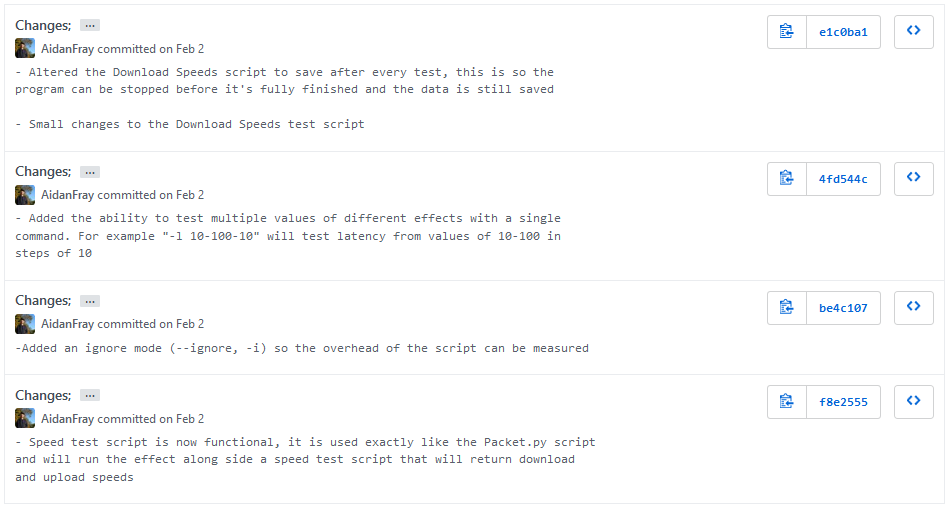
\includegraphics[scale=0.5]{github_commits}
	\begin{figure}[h]
		\caption{Sample of some commit messages used in the GitHub project}
		\label{ref:githubCommits}
	\end{figure}
\end{center}

%Further work:
%You should identify any specific areas of the existing product where further work is required, either to address known bugs or omissions, or to improve the system – for example an area you developed at an early stage may in hindsight have been structured in a better way, although it is still perfectly functional.
%You should also provide an outline of any additional areas of potential development you can envisage beyond the initial goals, where the system might be extended in future for greater functionality.
\section{Further work}
The project could be continued and improved in the ways discussed below.

\subsection{More protocols}
In the background there was discussion into the inclusion of other transport protocols or other TCP and UDP based protocols. This would give this project a much more in-depth analysis of more types of network traffic. QUIC would be a great addition to future goals of the project. QUIC is and incredibly new protocol and with the backing of Google gives it a higher chance of being adopted as a standard transfer protocol.

Testing and experiments could be performed to detect the effects of degradation such as latency and packet loss of this young protocol and could even contribute to the infant knowledge base.


\subsection{More platform support}
The tool is currently only supported on Linux. Therefore, further work could be to create version that run on Windows or Mac OS. This would allow the tool to be used for many more situations and on many more systems. This however would involve a large amount of work due to the differing ways that each OS would deal with firewall based packet filtering.


\subsection{Larger test network}
Another further improvement would be to use a more powerful router to host the script. Increased speed would allow support for a larger synthetic test network with more clients. Therefore, would provide more possible feedback because of the further improved realism and size of the test network. This improvement is mainly limited by the processing power of the computer used to host the script. 

This also touches on the possible improvement of the efficiency of the script, the use of a more embedded orientated language would provide a sizeable increase. A language similar to C or C++ would be suitable, this however, would be time consuming and library support would not be a comprehensive as Python's. Therefore, resulting in more time required to port the tool.